\documentclass[11pt]{article}
\usepackage[margin=1in]{geometry}
\usepackage{amsmath, amssymb}
\usepackage{graphicx}
\usepackage{hyperref}
\usepackage{booktabs}
\usepackage{float}

\title{CS336 Assignment 3 (scaling): Scaling Laws}
\author{Lenard Strahringer \\ Student ID: 06773780}
\date{Spring 2026}

\begin{document}

\maketitle

% ============================================================
\section{IsoFLOPs Scaling Laws (\texttt{chinchilla\_isoflops})}
% ============================================================

\subsection*{(a) Optimal Model Size}

\begin{figure}[H]
    \centering
    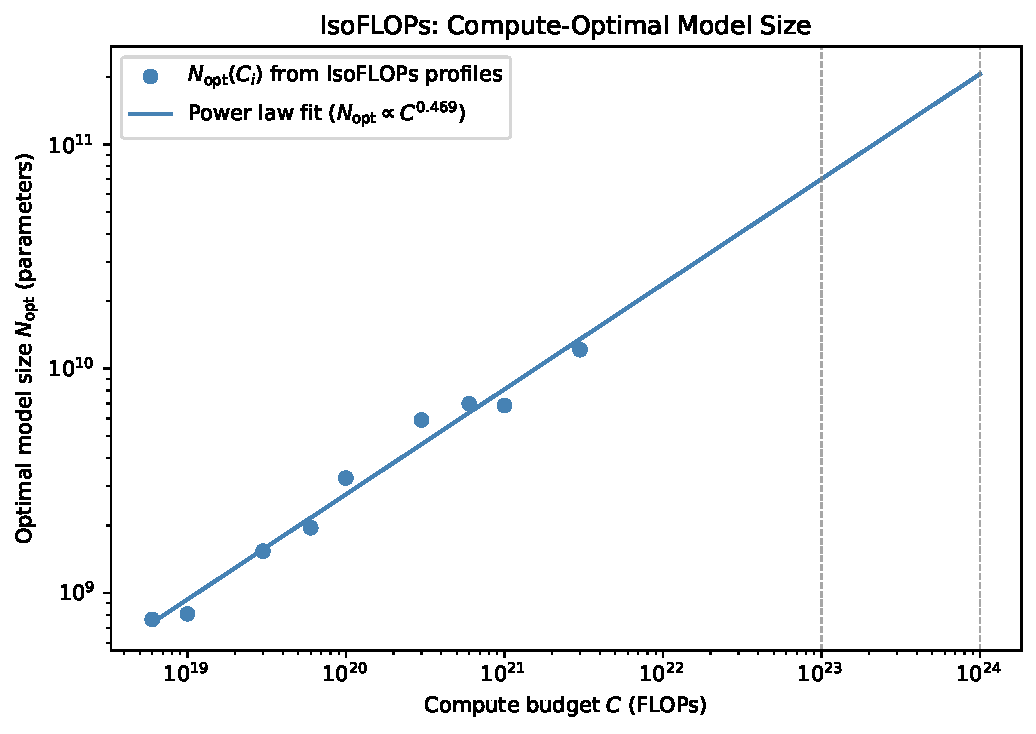
\includegraphics[width=0.75\textwidth]{figures/model_size_scaling.pdf}
    \caption{Compute-optimal model size $N_\text{opt}$ as a function of compute budget $C$.
    Data points show $\langle C_i, N_{\text{opt}(C_i)}\rangle$ from the IsoFLOPs profiles;
    the curve shows the fitted power law $N_\text{opt} \propto C^a$.}
    \label{fig:model-size-scaling}
\end{figure}

The optimal model size is $7.0 \times 10^{10}$ parameters at $C = 10^{23}$ FLOPs and $2.1 \times 10^{11}$ parameters at $C = 10^{24}$ FLOPs.

\subsection*{(b) Optimal Dataset Size}

\begin{figure}[H]
    \centering
    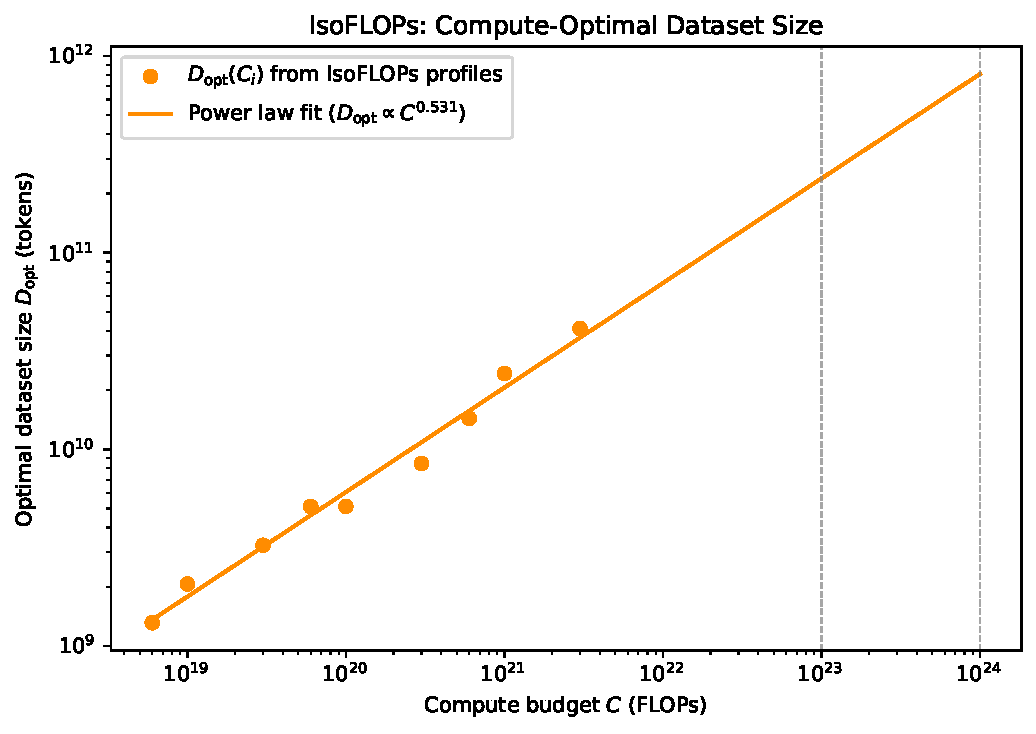
\includegraphics[width=0.75\textwidth]{figures/dataset_size_scaling.pdf}
    \caption{Compute-optimal dataset size $D_\text{opt}$ as a function of compute budget $C$.
    Data points show $\langle C_i, D_{\text{opt}(C_i)}\rangle$ from the IsoFLOPs profiles;
    the curve shows the fitted power law $D_\text{opt} \propto C^b$.}
    \label{fig:dataset-size-scaling}
\end{figure}

The optimal dataset size is $2.4 \times 10^{11}$ tokens at $C = 10^{23}$ FLOPs and $8.1 \times 10^{11}$ tokens at $C = 10^{24}$ FLOPs.

% ============================================================
\section{Constructing Scaling Laws (\texttt{scaling\_laws})}
% ============================================================

\subsection{Experimental Design}

[PLACEHOLDER: describe how you allocated your 12 B200-hour scaling-law budget --- which model sizes, token counts, and hyperparameter settings you queried, and why.]

\subsection{Fitting the Scaling Law}

[PLACEHOLDER: describe the method used to fit the scaling law (e.g.\ IsoFLOPs / Chinchilla approach, power-law fit via \texttt{scipy.optimize.curve\_fit}, etc.) and any design decisions made.]

\subsection{Quality of Fit}

\begin{figure}[H]
    \centering
    % 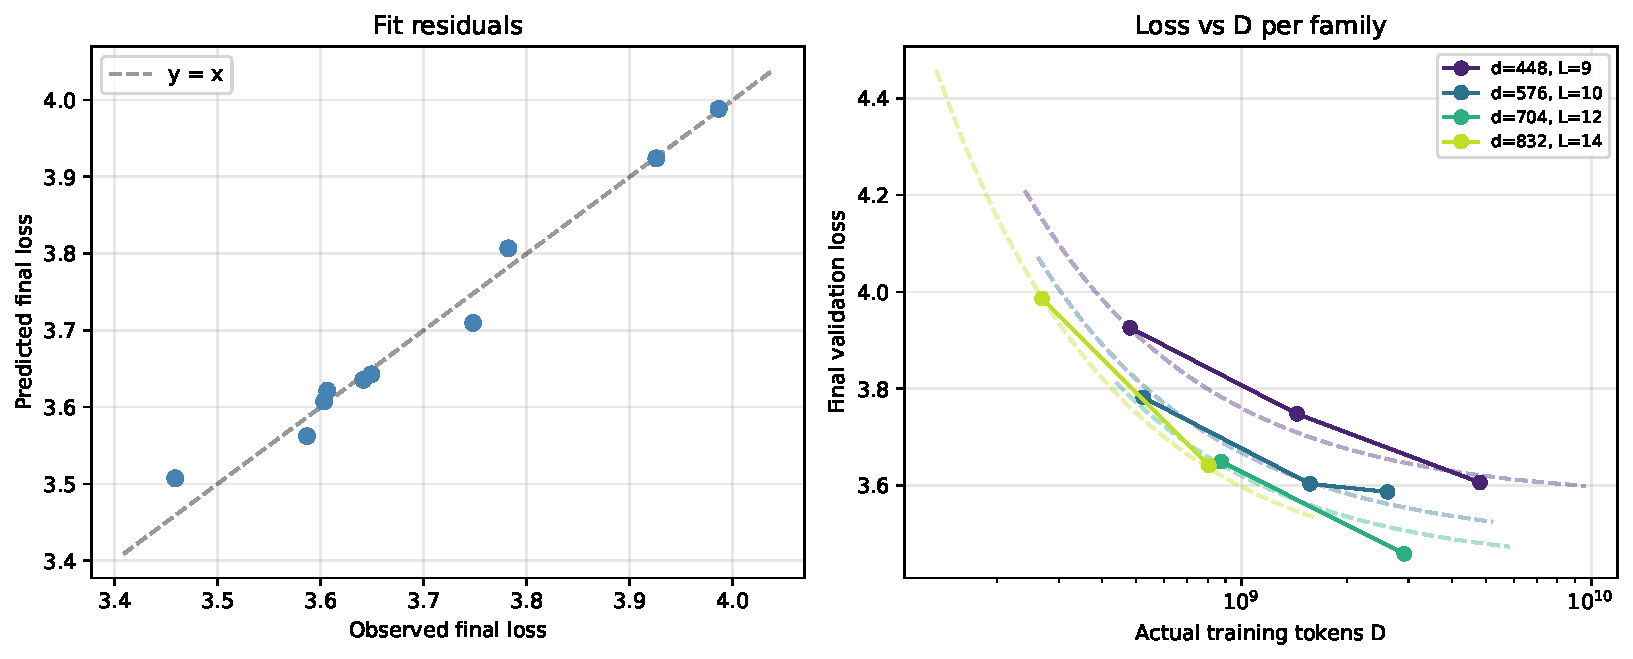
\includegraphics[width=0.75\textwidth]{figures/scaling_law_fit.pdf}
    \fbox{\parbox{0.75\textwidth}{\centering [PLACEHOLDER: plot showing fitted scaling law against experimental data points]}}
    \caption{Fitted scaling law overlaid on experimental validation losses.}
    \label{fig:scaling-law-fit}
\end{figure}

[PLACEHOLDER: brief quantitative assessment of how well the scaling law fits the data (e.g.\ $R^2$, residuals).]

\subsection{Predicted Optimal Configuration for 48 B200-Hours}

[PLACEHOLDER: state your predicted optimal model size $N^*$ and the predicted validation loss for the 48 B200-hour run.]

The predicted compute-optimal number of parameters is $N^* = \text{[PLACEHOLDER]}$, corresponding to a predicted final validation loss of $L^* = \text{[PLACEHOLDER]}$.

\subsection{Hyperparameter Choices}

[PLACEHOLDER: describe the architecture and optimizer hyperparameters you would use for the predicted optimal model. Justify choices (learning rate, batch size, number of layers, hidden size, etc.), referencing any smaller-scale experiments you ran to inform them. Recall that the non-embedding parameter count is approximated by $12 n_\text{layer} d_\text{model}^2$.]

\begin{table}[H]
    \centering
    \begin{tabular}{ll}
        \toprule
        Hyperparameter & Value \\
        \midrule
        \texttt{num\_hidden\_layers}   & [PLACEHOLDER] \\
        \texttt{hidden\_size}          & [PLACEHOLDER] \\
        \texttt{num\_attention\_heads} & [PLACEHOLDER] \\
        \texttt{head\_dim}             & [PLACEHOLDER] \\
        \texttt{intermediate\_size}    & [PLACEHOLDER] \\
        \texttt{total\_train\_tokens}  & [PLACEHOLDER] \\
        \texttt{train\_batch\_size}    & [PLACEHOLDER] \\
        Peak learning rate             & [PLACEHOLDER] \\
        \bottomrule
    \end{tabular}
    \caption{Predicted optimal hyperparameters for the 48 B200-hour run.}
    \label{tab:hyperparameters}
\end{table}

% ============================================================
\bibliographystyle{plain}
\begin{thebibliography}{9}

\bibitem{kaplan2020}
J.\ Kaplan \textit{et al.}, ``Scaling Laws for Neural Language Models.'' 2020.

\bibitem{hoffmann2022}
J.\ Hoffmann \textit{et al.}, ``Training Compute-Optimal Large Language Models.'' 2022.

\bibitem{yang2022}
G.\ Yang \textit{et al.}, ``Tensor Programs V: Tuning Large Neural Networks via Zero-Shot Hyperparameter Transfer.'' 2022.

\end{thebibliography}

\end{document}
